\begin{center}
    {\LARGE \textbf{2018物理化学}} \\[2ex]
    {\large 时量180分钟 \quad 满分150分}
\end{center}

\vspace{0.5cm}
\noindent\textbf{注意事项:}
\begin{enumerate}[label=\arabic*., parsep=0pt, itemsep=0pt]
    \item 答题前,考生先将自己的姓名、学号、考场号、座位号填写在答题卡上,将条形码准确粘贴在考生信息条形码粘贴区。
    \item 考试结束后,将本试卷与答题纸一并收回。
    \item 回答各个问题时,将答案写在答题纸上,写在本试卷上无效。
\end{enumerate}

\vspace{0.5cm}
\noindent\textbf{一、选择题（30 pts.）}

\begin{enumerate}[label=\arabic*., itemsep=1.5ex]
    \item 下面四种电解质溶液,浓度均为$0.01\mathrm{mol\cdot dm^{-3}}$，现已按它们的摩尔电导率$A_m$值由大到小排了次序.请根据你已有的知识,判定下面哪个是正确的?
    \begin{tasks}(1)
        \task $NaCl > KCl > KOH > HCl$
        \task $HCl > KOH > KCl > NaCl$
        \task $HCl > NaCl > KCl > KOH$
        \task $HCl > KOH > NaCl > KCl$
    \end{tasks}
    \item 若一气体的方程为$pV_m=RT+ap(a>0$常数$)$,则:
    \begin{tasks}(4)
        \task $\left(\dfrac{\partial U}{\partial V}\right)_T=0$
        \task $\left(\dfrac{\partial U}{\partial p}\right)_V=0$
        \task $\left(\dfrac{\partial U}{\partial T}\right)_V=0$
        \task $\left(\dfrac{\partial U}{\partial V}\right)_p=0$
    \end{tasks}
    \item 关于偏摩尔量,下面的叙述中不正确的是
    \begin{tasks}(1)
        \task 偏摩尔量的数值可以是正数、负数和零
        \task 溶液中每一种量度性质都有偏摩尔量,而且都不等于其摩尔量
        \task 除偏摩尔吉布斯自由能外,其他偏摩尔量都不等于化学势
        \task 溶液中各组分的偏摩尔量之间符合吉布斯—杜亥姆关系式
    \end{tasks}
    \item 现有四种处于相同温度和压力下的理想稀溶液
    \begin{enumerate}[label=(\arabic*), noitemsep, topsep=0pt, partopsep=0pt]
        \item $0.1\mathrm{mol}$蔗糖溶于 $80\mathrm{mol}$ 水中,水蒸气压力为$p_1$
        \item $0.1\mathrm{mol}$萘溶于 $80\mathrm{mol}$ 苯中,苯蒸气压力为$p_2$
        \item $0.1\mathrm{mol}$葡萄糖溶于$40\mathrm{mol}$ 水中,水蒸气压为 $p_3$
        \item $0.1\mathrm{mol}$尿素溶于 $80\mathrm{ml}$水中,水蒸气压为 $p_4$
    \end{enumerate}
    这四个蒸气压之间的关系为:
    \begin{tasks}(2)
        \task $p_1\neq p_2\neq p_3\neq p_4$
        \task $p_2\neq p_1=p_4>p_3$
        \task $p_1=p_2=p_4=(1/2)p_3$
        \task $p_1=p_4<2p_3\neq p_2$
    \end{tasks}
    \item $10^\circ C$时,苯甲酸在水中的溶解度 $S_1=0.207$ , $30^\circ C$时为$S_2=0.426$。每摩尔苯甲酸的平均溶解热为:
    \begin{tasks}(4)
        \task $6400J$
        \task $12000J$
        \task $25100J$
        \task $36740J$
    \end{tasks}
    \item 电导测定应用广泛,但下列问题中哪个是不能用电导测定来解决的?
    \begin{tasks}(2)
        \task 求难溶盐的溶解度
        \task 求弱电解质的解离度
        \task 求平均活度系数
        \task 测电解质溶液的浓度
    \end{tasks}
    \item 已知$Cu$的相对原子量为 $64$，用$0.5$法拉第电量可从$CuSO_4$溶液中沉淀出多少$Cu$?
    \begin{tasks}(4)
        \task $16g$
        \task $32g$
        \task $64g$
        \task $127g$
    \end{tasks}
    \item 自然界中,有的高大树种可以长到$100m$ 以上，能够提供营养及水位到树冠的主要动力是什么?
    \begin{tasks}(1)
        \task 因外界大气压引起的树干内导管的空吸作用
        \task 树干中微导管的毛细作用
        \task 树内体液含盐浓度高，渗透压大
        \task 营养和水分自雨水直接落到树冠上
    \end{tasks}
    \item 当体系将热量传递给环境之后,体系的焓：
    \begin{tasks}(4)
        \task 必定减少
        \task 必定增加
        \task 必定不变
        \task 不一定改变
    \end{tasks}
    \item 在$263K$的过冷水凝结成$263K$的冰,则
    \begin{tasks}(4)
        \task $\Delta S<0$
        \task $\Delta S>0$
        \task $\Delta S=0$
        \task 不能确定
    \end{tasks}
    \item 某具有简单级数的反应, $k=0.1dm^3\cdot mol^{-1}\cdot s^{-1}$起始浓度为$0.1mol\cdot dm^{-3}$当反应速率降至起始速率$1/4$时，所需时间为:
    \begin{tasks}(4)
        \task $0.1s$
        \task $333s$
        \task $30s$
        \task $100s$
    \end{tasks}
    \item 对于气相反应,当体系总压力$p$ 变化时
    \begin{tasks}(2)
        \task 对$K^\ominus$无影响
        \task 对$K_r$无影响
        \task 对$K_p^\ominus$无影响
        \task 对$K_f$、$K_r$、$K_p^\ominus$均无影响
    \end{tasks}
    \item 在$\alpha$、$\beta$两相中均含有$A$和$B$两种物质，当达到平衡时，下列哪种情况是正确的?
    \begin{tasks}(4)
        \task $\mu_A^\alpha=\mu_B^\alpha$
        \task $\mu_A^\alpha=\mu_A^\beta$
        \task $\mu_A^\alpha=\mu_B^\beta$
        \task $\mu_A^\beta=\mu_B^\beta$
    \end{tasks}
    \item 一定量的理想气体从同一始态出发,分别经（1）等温压缩，（2）绝热压缩到具有相同压力的终态，以$H_1$,$H_2$ 分别表示两个终态的焓值，则有
    \begin{tasks}(4)
        \task $H_1>H_2$
        \task $H_1=H_2$
        \task $H_1<H_2$
        \task $H_1\geq H_2$
    \end{tasks}
    \item 两个活化能不相同的反应，如$E_2>E_1$，且都在相同的升温度区间内升温，则：
    \begin{tasks}(2)
        \task $\dfrac{d\ln k_2}{dT}>\dfrac{d\ln k_1}{dT}$
        \task $\dfrac{d\ln k_2}{dT}<\dfrac{d\ln k_1}{dT}$
        \task $\dfrac{d\ln k_2}{dT}=\dfrac{d\ln k_1}{dT}$
        \task $\dfrac{dk_2}{dT}>\dfrac{dk_1}{dT}$
    \end{tasks}
\end{enumerate}

\vspace{0.5cm}
\noindent\textbf{二、计算题（20 pts.）}

$1\mathrm{mol}$单原子分子理想气体经过一个绝热不可逆过程到达终态,该终态的温度为$273K$，压力为$p^\ominus$,熵值为$S_m^s(273K)=188.3J\cdot K^{-1}\cdot mol^{-1}$，已知该过程$W=1255J$，$\Delta S_m=-20.92J\cdot K^{-1}\cdot mol^{-1}$
\begin{enumerate}[label=(\arabic*), itemsep=1ex]
    \item 求始态的的 $P_1,V_1,T_1$；
    \item 求气体的 $\Delta U,\Delta H,\Delta G$
\end{enumerate}

\vspace{0.5cm}
\noindent\textbf{三、计算题（15 pts.）}

$298.15K$时液态乙醇的摩尔标准熵为 $160.7J\cdot K^{-1}mol^{-1}$,蒸气压是$7.866kPa$,汽化热为 $42.635KJ\cdot mol^{-1}$。

计算标准压力$p^\ominus$下$298.15K$ 时乙醇蒸气的摩尔标准熵。假定乙醇蒸气为理想气体。

\vspace{0.5cm}
\noindent\textbf{四、计算题（15 pts.）}

液体$A$和$B$可形成理想液态混合物。把组成为 $y_A=0.400$的二元蒸气混合物放入一带有活塞的气缸中进行恒温压缩。已知该温度时$p_A^*$和$p_B^*$分别为$40530Pa$ 和 $121590Pa$。
\begin{enumerate}[label=(\arabic*), itemsep=1ex]
    \item 计算刚开始出现液相时的蒸气总压；
    \item 求$A$ 和$B$ 的液态混合物在上述温度和$101325Pa$下沸腾时液相的组成。
\end{enumerate}

\newpage

\vspace{0.5cm}
\noindent\textbf{五、计算题（15 pts.）}

指出下面$a$,$b$两图中所形成的化合物的经验式,并说明各相区是由哪些相组成的

\begin{figure}[htbp]
    \centering
    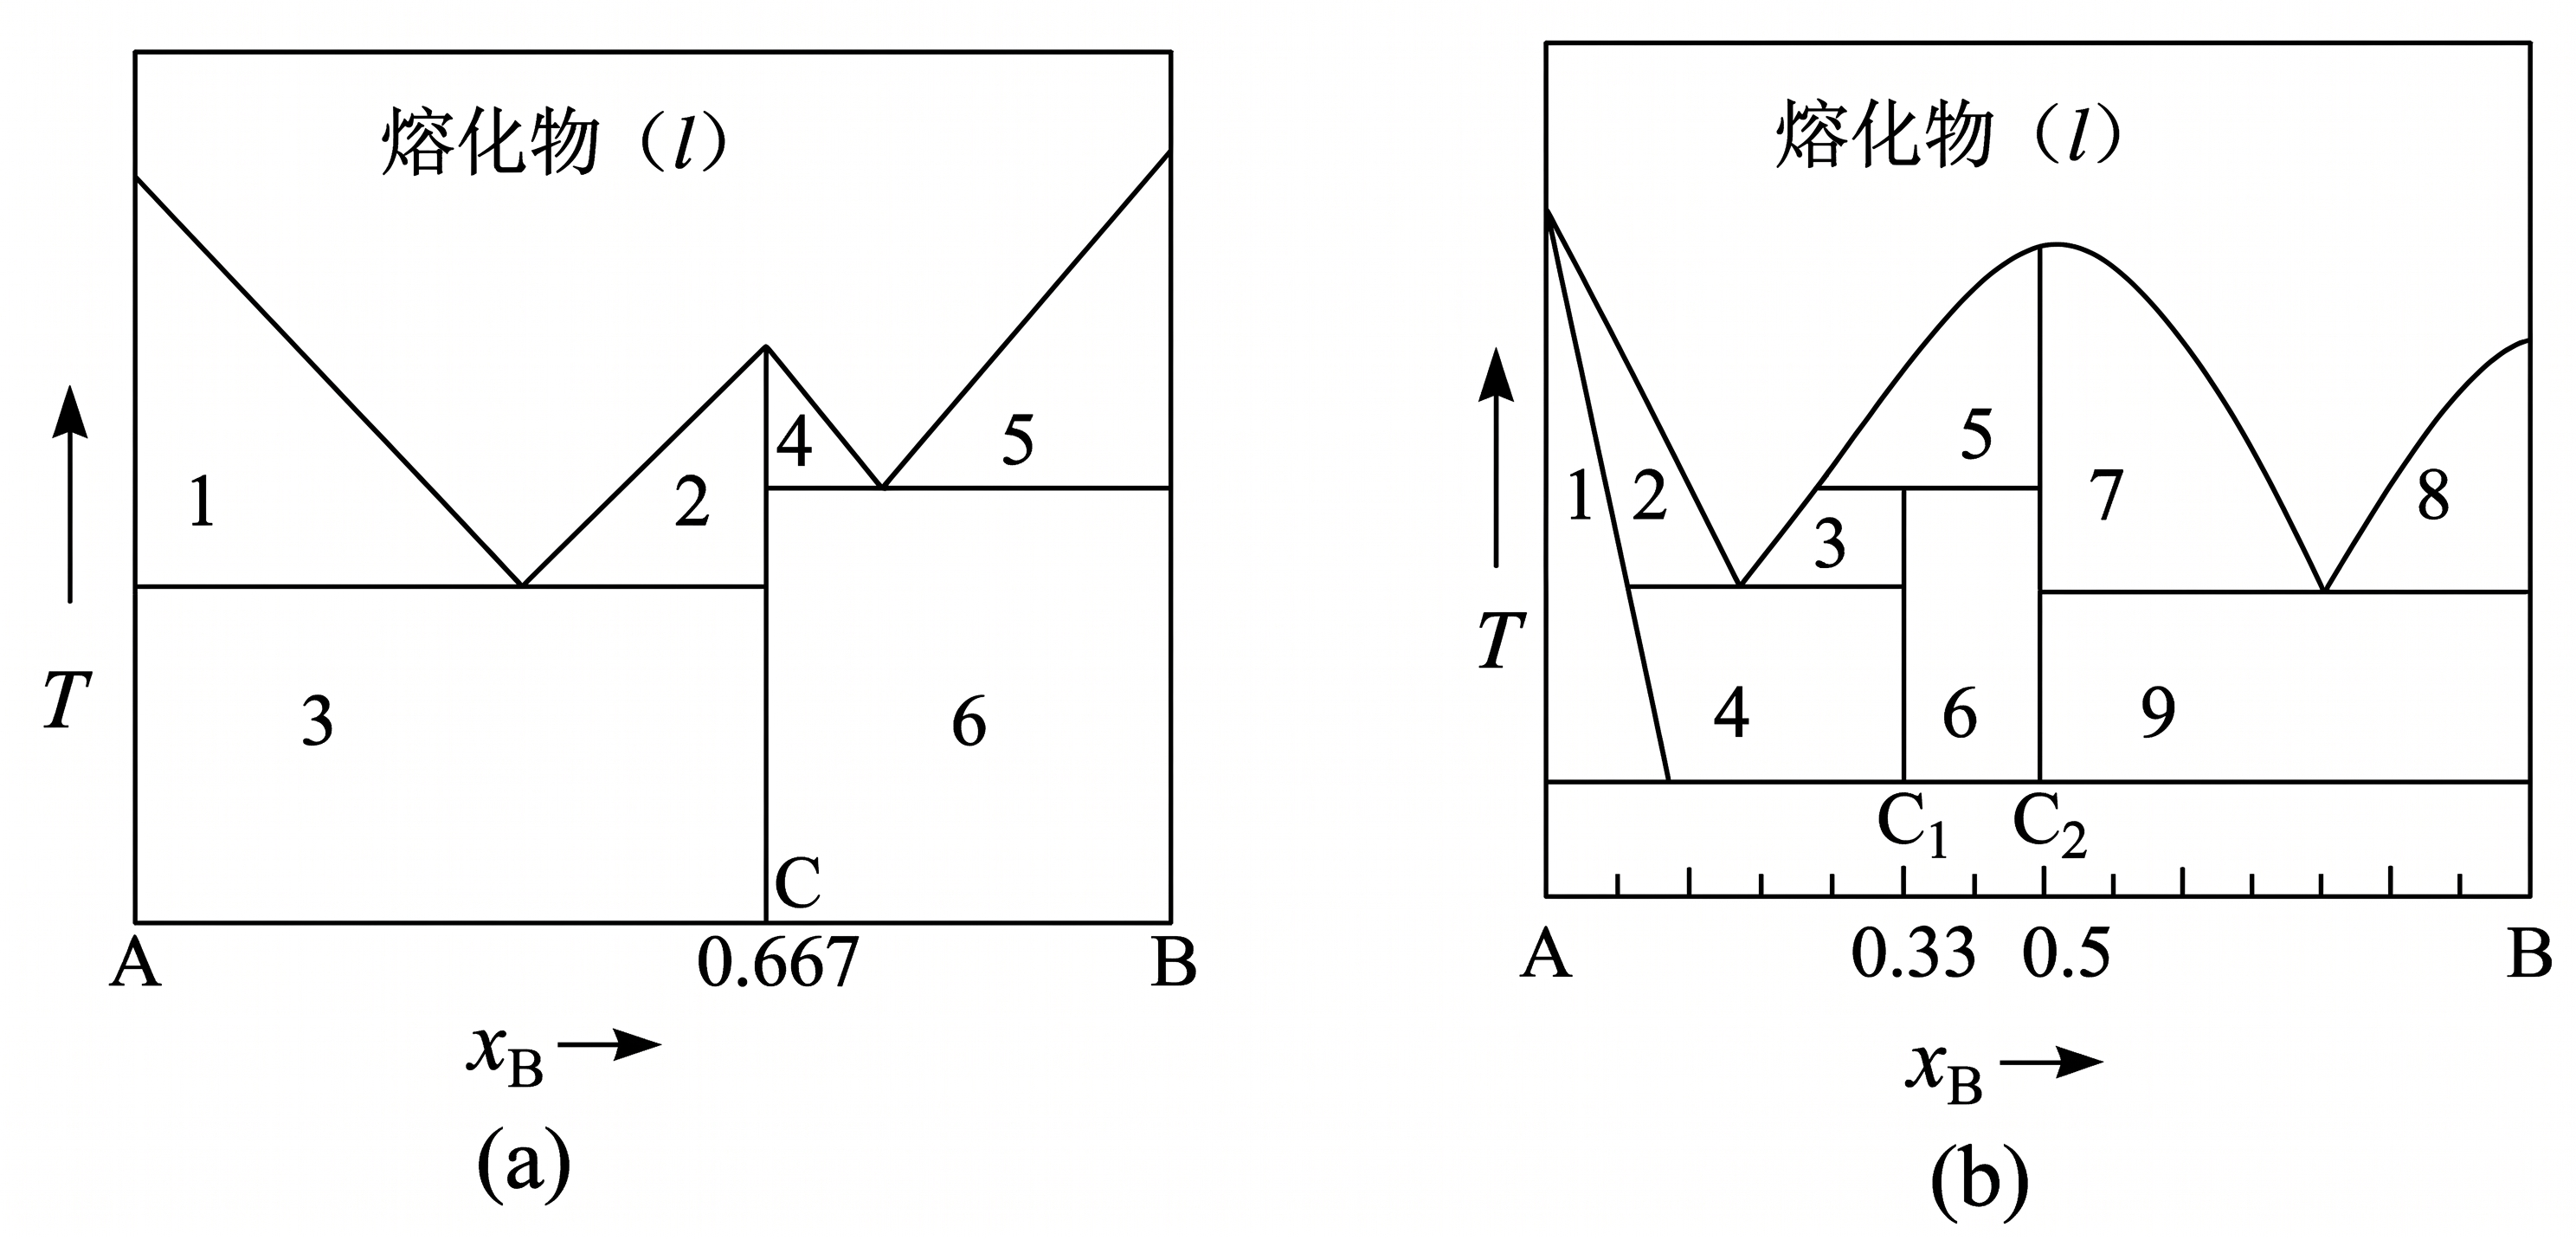
\includegraphics[width=0.8\textwidth]{./Figure/P_2018_5}

\end{figure}

\vspace{0.5cm}
\noindent\textbf{六、计算题（15pts.）}

$\ce{CO2}$在高温时按下式分解 $2\ce{CO2}\rightarrow 2\ce{CO}+\ce{O2}$,在$p^\ominus$,$1000K$ 时解离度为 $2.0\times10^{-7}$，$1400K$ 时为$1.27\times10^{-4}$,设在该温度范围内反应热效应不随温度而改变,则在 $1000K$ 时反应的$\Delta_rG_m$和$\Delta_rS_m$各为多少?

\vspace{0.5cm}
\noindent\textbf{七、计算题（20 pts.）}

对某一特定的一级反应在 $27^\circ C$反应时,经过$5000s$ 后, 反应物的浓度减少到初始值的一半，在$37^\circ C$时，经过$1000s$，浓度就减半，计算：
\begin{enumerate}[label=(\arabic*), itemsep=1ex]
    \item $27^\circ C$时的反应速率常数；
    \item 在$37^\circ C$反应时,当反应物浓度降低到其初始值的四分之一时所需的时间；
    \item 该反应的活化能。
\end{enumerate}

\vspace{0.5cm}
\noindent\textbf{八、计算题（20 pts.）}

$298K$时有电池$\ce{Pt,H2(p^\ominus)|KOH(\alpha=1),Ag2O(s)|Ag(s)}$，
已知 $E(\ce{Ag2O|Ag})=0.344V$
$\Delta_fH_m(\ce{H2O,l})=286.0kJ\cdot mol^{-1}$ $\Delta_fH_m(\ce{Ag2O,s})=30.57kJ\cdot mol^{-1}$（标准状态下）试求:
\begin{enumerate}[label=(\arabic*), itemsep=1ex]
    \item 电池的电动势已知$K_w=1.0\times10^{-14}$
    \item 电池反应的$\Delta_rG_m^\ominus,\Delta_rH_m^\ominus,\Delta_rS_m^\ominus,Q_r$和$\left(\dfrac{\partial E}{\partial T}\right)_p$
    \item 若电池在短路下放电,程度与可逆反应相同时,求热效应为多少
\end{enumerate}